\chapter{Anexos}
%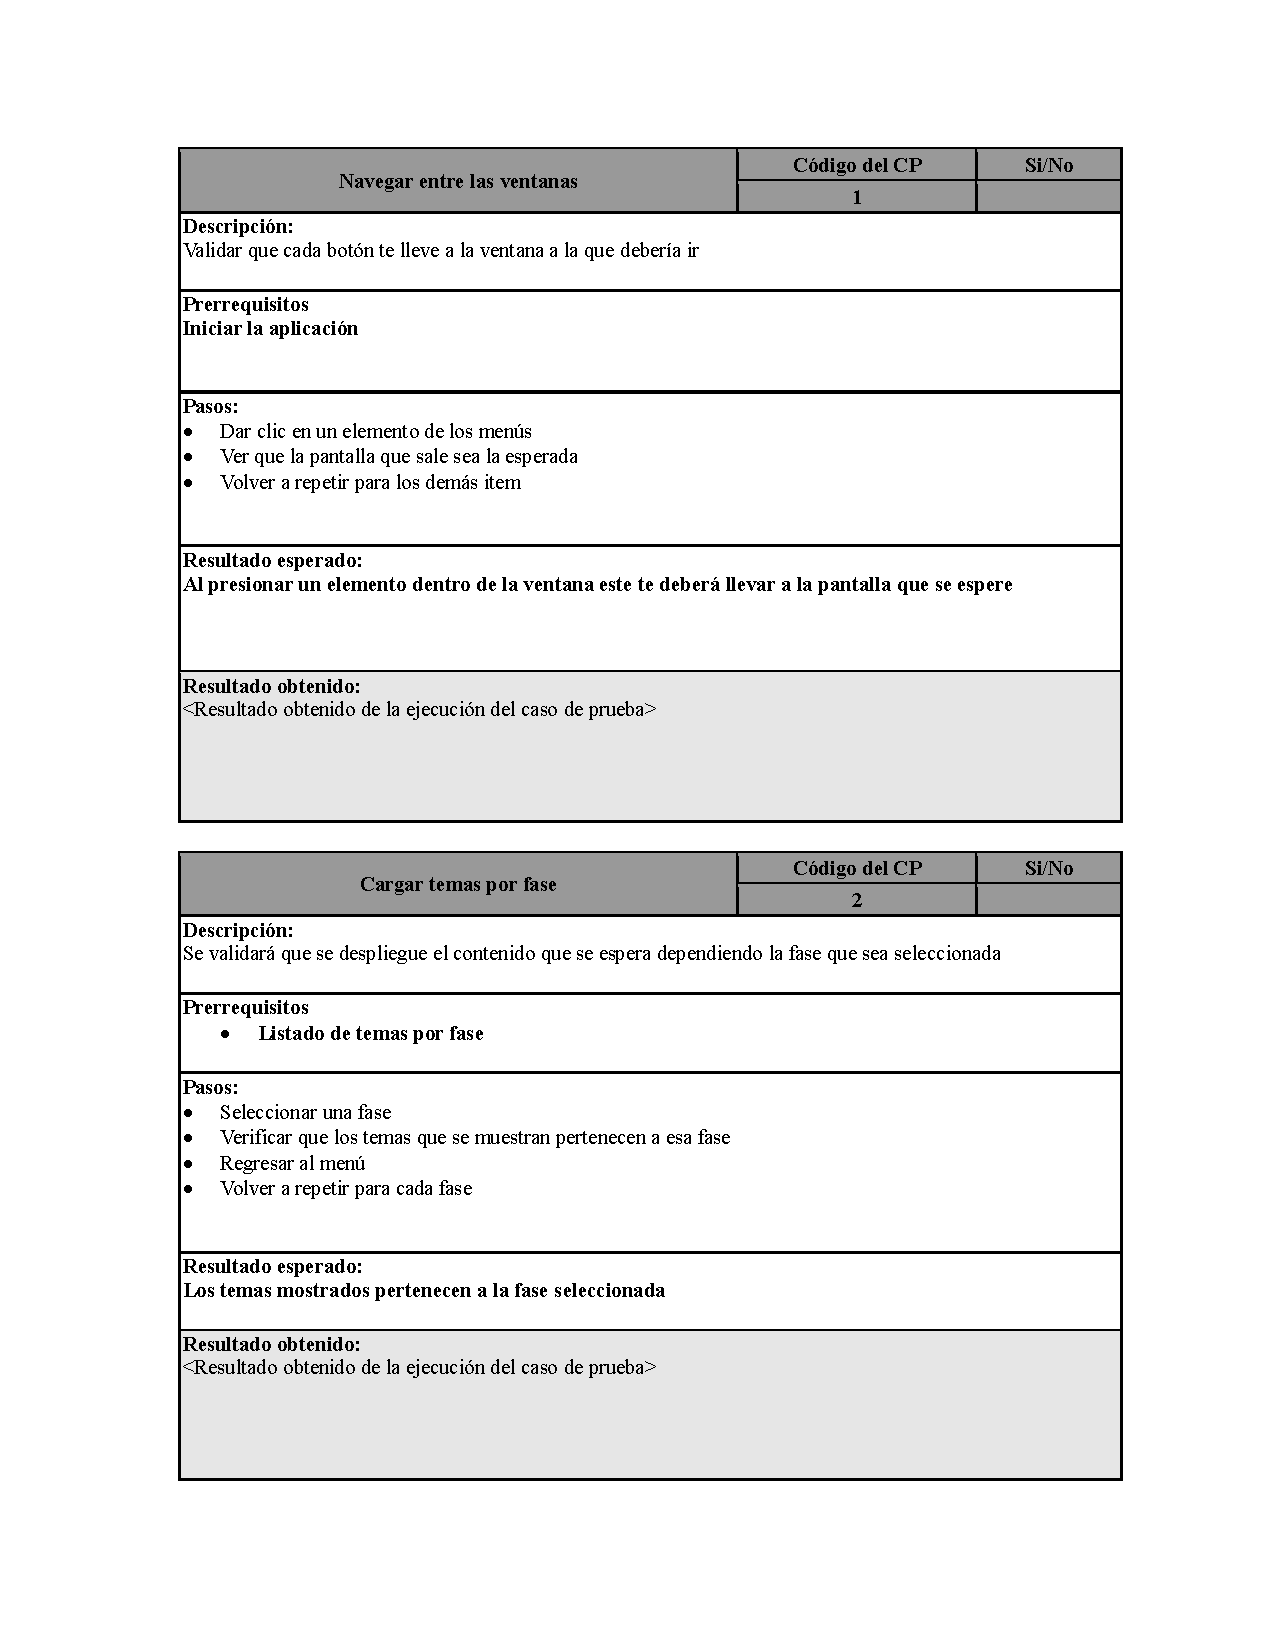
\includepdf[pages=-]{cdp}
\section{Plan de pruebas}
El plan de pruebas es el documento fundamental en torno al cual se desarrollan las pruebas.
Un plan de pruebas explica cómo el conjunto de pruebas debe ser usado y el soporte necesario para realizar el proceso de pruebas. Describe alcance, enfoque, recursos y calendarización de actividades de prueba. Identifica las tareas de prueba a desarrollar, los responsables de cada tarea y los riesgos asociados. Generalmente un plan de pruebas es un documento bastante extenso y debe organizarse para que sea entendible y mantenible.
Para esto se propone el estándar IEEE 829 de Documentación el cual provee una tabla de contenidos para documentar un conjunto de pruebas.

\begin{longtable}[c]{|l|l|}
\hline
IEE 829 & Contenido \\ \hline
\endfirsthead
%
\endhead
%
\begin{tabular}[c]{@{}l@{}}Plan\\ de Pruebas CodeLandOOP\end{tabular} & \begin{tabular}[c]{@{}l@{}}-Items a probar\\    *Menú Fases\\    *Menú Temas\\    *Cuestionario\\    *Ejercicio\\    *Ejemplo\\    *Información mostrada al usuario\\ -Textbox\\ -Labels\\ -Combobox\\ -Botones\\ Características a ser probadas.\\ -Que los botones realizaran las\\ acciones para los que estaban diseñados  \\ -Que los Labels tuvieran una buena\\ ortografía\\ -Requerimientos funcionales\\ -Requerimientos no funcionales\\ -Que tenga configurada una buena\\ tabulación.\\ -Adaptable a cualquier resolución\\ Características que no se van a probar \\ -Compatibilidad en IOS\end{tabular} \\ \hline
Enfoque & \begin{tabular}[c]{@{}l@{}}Este plan de pruebas es necesario para\\ el aseguramiento de la calidad del sistema. \\ Con este plan se seleccionan y se coordinan \\ las actividades para asegurar la calidad del \\ software durante el ciclo de vida del proyecto \\ y aún después al ser entregado al cliente. Los \\ objetivos que se pretenden alcanzar con la \\ aplicación del plan de pruebas son\\ \\ las siguientes:\\ \\ -Encontrar la mayor cantidad de errores como\\ sea posible, ya sea tanto en los TextBox, como\\  la ortografía que hay en las Labels, los botones,\\  los ComboBox.\\ -Supervisar si se cumple las especificaciones de\\  diseño establecidas por el cliente.\\ -Supervisar si se cumple los requisitos del \\ análisis que se hicieron en la planificación\\  del diseño y desarrollo del software. \\ -Realizar pruebas las pruebas necesarias de \\ rendimiento y capacidad del sistema.\\ -Encontrar los problemas importantes y \\ determinar los riesgos percibidos en cuanto\\  a la calidad del producto.\\ Los tipos de pruebas que se realizarán\\ al software son:\\ -Pruebas de Función\\ -Pruebas de Interfaces de usuario \\ -Pruebas de Desempeño\end{tabular} \\ \hline
Casos de prueba &  \\ \hline
Tareas y responsabilidades & \begin{tabular}[c]{@{}l@{}}Administrador del plan de pruebas (análisis)\\ -Definición de casos de prueba\\ -Resumen del ciclo de prueba (resultados y observaciones)\\ Desarrolladores o personal de ejecución de pruebas\\ -Pruebas de Función\\ -Pruebas de Interfaces de usuario \\ -Pruebas de Desempeño\end{tabular} \\ \hline
Requerimientos de ambiente & \begin{tabular}[c]{@{}l@{}}La aplicación se puede ejecutar\\ perfectamente en un dispositivo que contenga \\ un procesador equivalente a 2.6\\ Ghz y 256 MB en RAM.\\ \\ Se requiere que para la prueba se cuente con el\\ SO Android en cualquiera de sus distintas \\ versiones, así como la instalación de\\ la aplicación CodeLandOOP.\end{tabular} \\ \hline
Personal necesario y entrenamiento & \begin{tabular}[c]{@{}l@{}}A nivel personal, se requiere atención por el \\ detalle, concentración, organización y capacidad\\  para analizar los resultados de las pruebas en\\ busca de soluciones.\\ Este trabajo implica la colaboración con otros\\ profesionales, por lo que saber trabajar en \\ equipo será fundamental.\\ \\ En cuanto a los aspectos técnicos cabe destacar\\ que los lenguajes de programación que este \\ profesional debería aprender para corregir\\ errores y ejecutar pruebas variarán dependiendo\\ del área en que se especialice.\\ Sin embargo, el manejo de lenguaje Java y XML\\ son necesarios en conjunto con Android Studio.\end{tabular} \\ \hline
Planificación & \begin{tabular}[c]{@{}l@{}}De acuerdo a la planificación descrita en el \\ diagrama de gantt el tiempo para realizar las\\ pruebas es de 4 días, el cual se extenderá en caso\\ de encontrar problemas, al aplicar las medidas \\ necesarias se planificará el siguiente ciclo de\\  pruebas a aplicar.\end{tabular} \\ \hline
Riesgos y contingencias & \begin{tabular}[c]{@{}l@{}}Los problemas que se encuentren en el proceso\\ serán documentados y al igual que los problemas\\ se documentarán las soluciones de éstos, el \\ proceso que se seguirá para alcanzar la resolución\\ de dichos problemas será el ir identificando cada\\ uno de los problemas y aplicar las medidas \\ necesarias para la solución de éstos.\end{tabular} \\ \hline
Aprobación & \begin{tabular}[c]{@{}l@{}}Encargado del plan de pruebas, realizará \\ resumen del ciclo de prueba (resultados y \\ observaciones), y dará su aprobación si se\\  obtuvieron resultados positivos de todos los\\ casos de prueba y no hubo errores sin resolver \\ de Gravedad. Esto demuestra la consecución \\ de los objetivos de las pruebas, con lo que la \\ solución está lista para el lanzamiento.\end{tabular} \\ \hline
\end{longtable}
\section{Casos de pruebas}
\begin{table}[H]\small
\begin{tabular}{@{\extracolsep{\fill}} |p{9cm}|p{4cm}|p{2cm}|}
\hline
\textbf{1. Navegar entre las ventanas} & \textbf{Código del CP:} 1& \textbf{Si / No} \\ \hline
\multicolumn{3}{|p{15cm}|}{\textbf{Descripción:}

Validar que e botón te lleve a la ventana que debería ir.} \\ \hline
\multicolumn{3}{|p{15cm}|}{Prerequisitos:

Iniciar la aplicación.} \\ \hline
\multicolumn{3}{|p{15cm}|}{\textbf{Pasos:}
\begin{itemize}
	\item Dar click en un elemento de los menús.
	\item Ver que la pantalla que sale sea la esperada.
	\item Volver a repetir para los demás item
\end{itemize}}\\ \hline
\multicolumn{3}{|p{15cm}|}{\textbf{Resultado esperado:}

Al presionar un elemento dentro de la ventana este te deberá llevar a la pantalla que se espere.} \\ \hline
\multicolumn{3}{|p{15cm}|}{\textbf{Resultado obtenido:}

<Resultado esperado de la ejecucion de la prueba>} \\ \hline
\hline
\end{tabular}
\caption{Caso de prueba numero 1}
\label{p1}
\end{table}
%%%%%%%%%%%%%%%%%%%%%%%%%%%%%%%%%%%%%%%%%%%%%%%%%%%%%%%%%%%%%%%%%%%%%%%%%%%%%%%%%%%%%
\begin{table}[H]\small
\begin{tabular}{@{\extracolsep{\fill}} |p{9cm}|p{4cm}|p{2cm}|}
\hline
\textbf{2. Cargar items por fases} & \textbf{Código del CP:} 2& \textbf{Si / No} \\ \hline
\multicolumn{3}{|p{15cm}|}{\textbf{Descripción:}

Se validará que se despliegue el contenido que se espera dependiendo de la fase que sea seleccionada.} \\ \hline
\multicolumn{3}{|p{15cm}|}{Prerequisitos:

Listado de temas por fase.} \\ \hline
\multicolumn{3}{|p{15cm}|}{\textbf{Pasos:}
\begin{itemize}
	\item Seleccionar una fase.
	\item Verificar que los items que se muestren pertenezcan a esa fase.
	\item Regresar al menú.
	\item Repetir los pasos anteriores para cada fase.
\end{itemize}}\\ \hline
\multicolumn{3}{|p{15cm}|}{\textbf{Resultado esperado:}

Los temas mostrados pertenecen a la fase seleccionada.} \\ \hline
\multicolumn{3}{|p{15cm}|}{\textbf{Resultado obtenido:}

<Resultado esperado de la ejecucion de la prueba>} \\ \hline
\hline
\end{tabular}
\caption{Caso de prueba numero 2}
\label{p2}
\end{table}
%%%%%%%%%%%%%%%%%%%%%%%%%%%%%%%%%%%%%%%%%%%%%%%%%%%%%%%%%%%%%%%%%%%%%%%%%%%%%%%%%%%%%
\begin{table}[H]\small
\begin{tabular}{@{\extracolsep{\fill}} |p{9cm}|p{4cm}|p{2cm}|}
\hline
\textbf{3. Cargar contenidos por temas} & \textbf{Código del CP:} 3& \textbf{Si / No} \\ \hline
\multicolumn{3}{|p{15cm}|}{\textbf{Descripción:}

Validar que se despliegue el contenido que se espera dependiendo el tema seleccionado.} \\ \hline
\multicolumn{3}{|p{15cm}|}{Prerequisitos:

Seleccionar una fase.} \\ \hline
\multicolumn{3}{|p{15cm}|}{\textbf{Pasos:}
\begin{itemize}
	\item Seleccionar un tema.
	\item Verificar que el contenido mostrado corresponda al tema.
	\item Regresar al listado de temas.
	\item Volver a repetir para cada tema.
\end{itemize}}\\ \hline
\multicolumn{3}{|p{15cm}|}{\textbf{Resultado esperado:}

Los contenidos mostrados pertnecen al tema seleccionado.} \\ \hline
\multicolumn{3}{|p{15cm}|}{\textbf{Resultado obtenido:}

<Resultado esperado de la ejecucion de la prueba>} \\ \hline
\hline
\end{tabular}
\caption{Caso de prueba numero 3}
\label{p1}
\end{table}
%%%%%%%%%%%%%%%%%%%%%%%%%%%%%%%%%%%%%%%%%%%%%%%%%%%%%%%%%%%%%%%%%%%%%%%%%%%%%%%%%%%%%
\begin{table}[H]\small
\begin{tabular}{@{\extracolsep{\fill}} |p{9cm}|p{4cm}|p{2cm}|}
\hline
\textbf{4. Mostrar información completa} & \textbf{Código del CP:} 3& \textbf{Si / No} \\ \hline
\multicolumn{3}{|p{15cm}|}{\textbf{Descripción:}

Se validará que se la información que se muestra sea toda la que debería aparecer.} \\ \hline
\multicolumn{3}{|p{15cm}|}{Prerequisitos:

Información de los temas.} \\ \hline
\multicolumn{3}{|p{15cm}|}{\textbf{Pasos:}
\begin{itemize}
	\item Seleccionar un tema.
	\item Verificar que el contenido mostrado no carezca de información.
	\item Regresar al listado de temas.
	\item Volver a repetir para cada tema.
\end{itemize}}\\ \hline
\multicolumn{3}{|p{15cm}|}{\textbf{Resultado esperado:}

La información mostrada es la misma que debería mostrarse.} \\ \hline
\multicolumn{3}{|p{15cm}|}{\textbf{Resultado obtenido:}

<Resultado esperado de la ejecucion de la prueba>} \\ \hline
\hline
\end{tabular}
\caption{Caso de prueba numero 4}
\label{p1}
\end{table}
%%%%%%%%%%%%%%%%%%%%%%%%%%%%%%%%%%%%%%%%%%%%%%%%%%%%%%%%%%%%%%%%%%%%%%%%%%%%%%%%%%%%%
\begin{table}[H]\small
\begin{tabular}{@{\extracolsep{\fill}} |p{9cm}|p{4cm}|p{2cm}|}
\hline
\textbf{5. Mostrar correctamente los tama'nos} & \textbf{Código del CP:} 5& \textbf{Si / No} \\ \hline
\multicolumn{3}{|p{15cm}|}{\textbf{Descripción:}

Se validará que se la información que se muestra sea toda la que debería aparecer.} \\ \hline
\multicolumn{3}{|p{15cm}|}{Prerequisitos:

Dispositivos con diferentes tamaños de pantalla.} \\ \hline
\multicolumn{3}{|p{15cm}|}{\textbf{Pasos:}
\begin{itemize}
	\item Instalar la apk.
	\item Navegar por las distintas pantallas.
	\item Verificar que en todas las pantallas se muestren correctamente iconos, botones, ítems, entre otros.
\end{itemize}}\\ \hline
\multicolumn{3}{|p{15cm}|}{\textbf{Resultado esperado:}

Los iconos y demás elementos se encuentran en los lugares esperados.} \\ \hline
\multicolumn{3}{|p{15cm}|}{\textbf{Resultado obtenido:}

<Resultado esperado de la ejecucion de la prueba>} \\ \hline
\hline
\end{tabular}
\caption{Caso de prueba numero 5}
\label{p1}
\end{table}
%%%%%%%%%%%%%%%%%%%%%%%%%%%%%%%%%%%%%%%%%%%%%%%%%%%%%%%%%%%%%%%%%%%%%%%%%%%%%%%%%%%%%